\documentclass[thesis.tex]{subfiles}
\begin{document}

\section{Introduction}
\label{sec:introduction}

In the field of computer vision, researchers have for many years tried to make computers interpret real world images as humans do. We have chosen to focus on two problems within this field: image correspondence \cite{dahl2011finding}, where we search for corresponding points between two different images taken of the same object, and pedestrian detection \cite{felzenszwalb2008discriminatively}, where locations of pedestrians are identified. These objectives are illustrated in \Cref{fig:introduction}. The approaches to these problems are often based on creating descriptors to represent regions of the images, and comparing these descriptors by some method depending on the application. Popular and successful descriptors include the SIFT \cite{lowe2004distinctive}, GLOH \cite{mikolajczyk2005performance}, DAISY \cite{tola2008fast}, and HOG \cite{dalal2005histograms,felzenszwalb2009object}. \todo{add "descriptors"?}
%
\begin{figure}[tb]
\centering
	\centerline{\begin{subfigure}[t]{0.51\textwidth}
		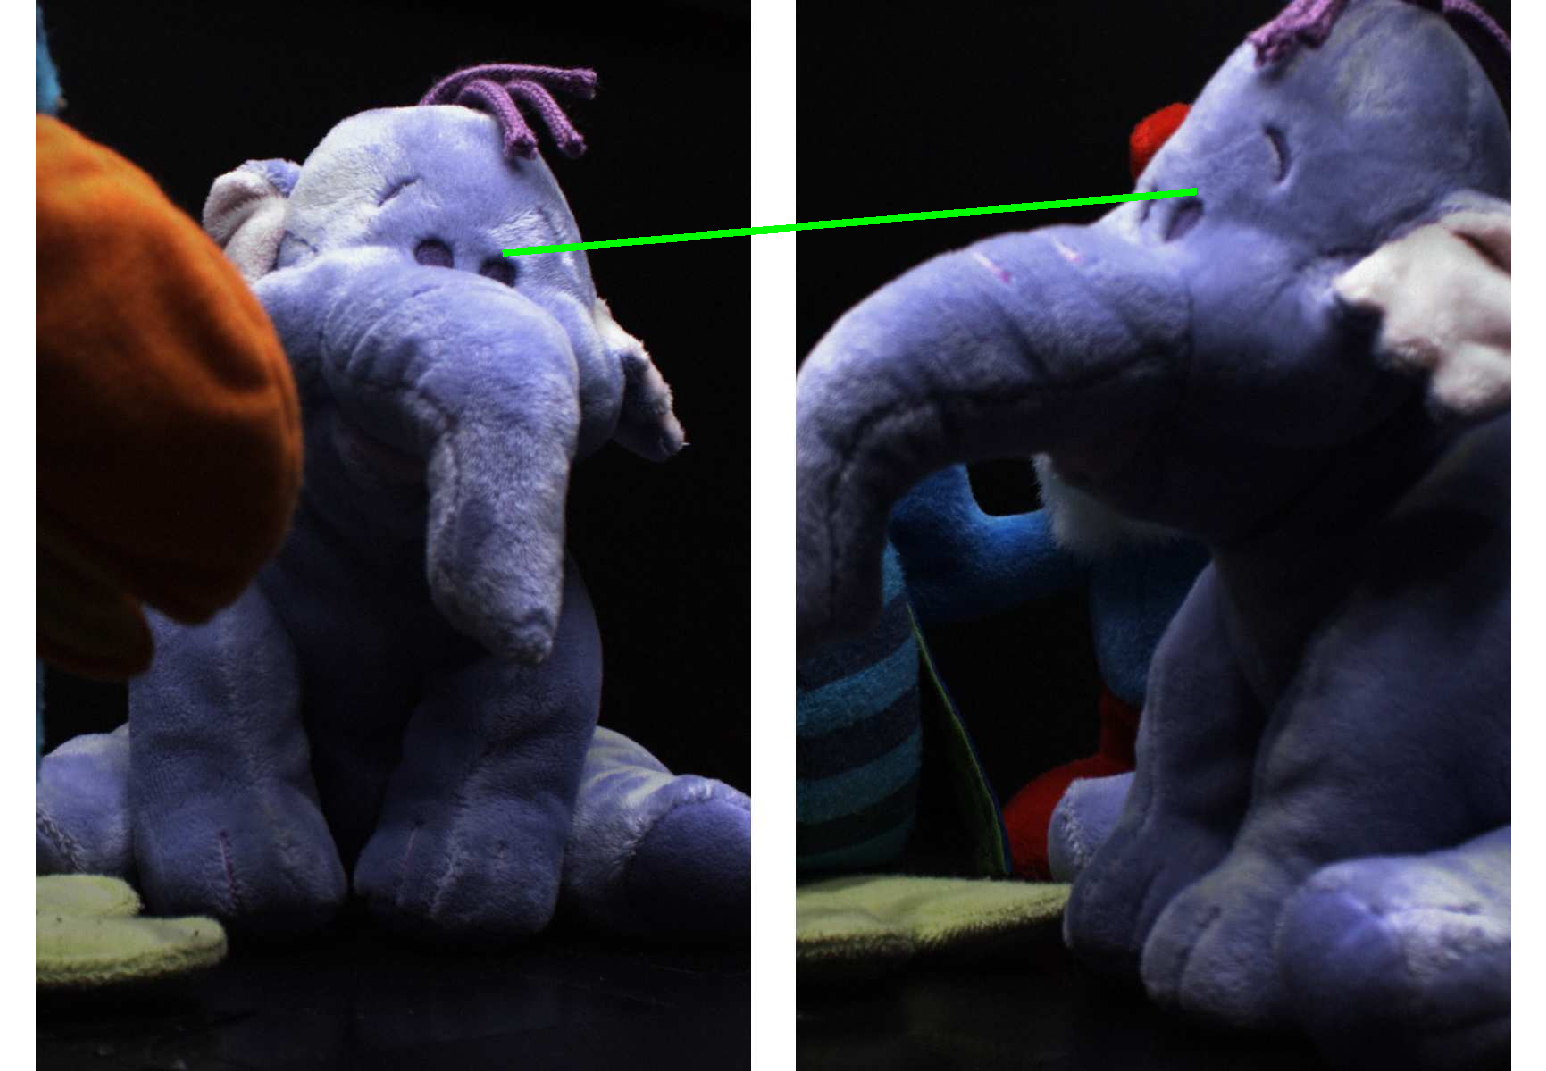
\includegraphics[width=\textwidth]{img/introductionIC.pdf}
		\caption{Image correspondence}
		\label{fig:introductionIC}
	\end{subfigure}
	\begin{subfigure}[t]{0.51\textwidth}
		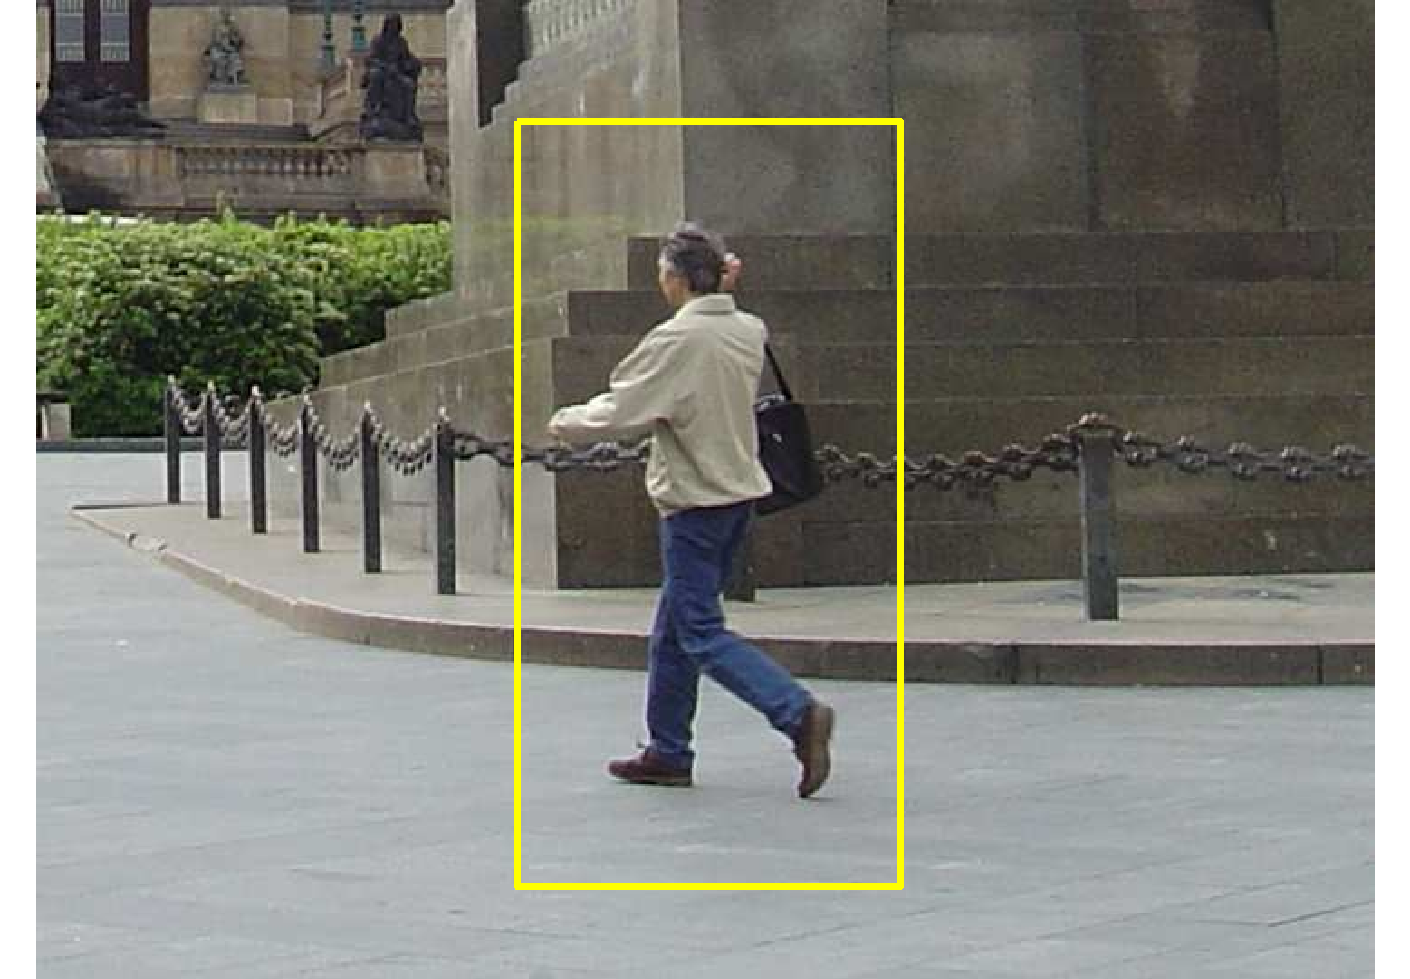
\includegraphics[width=\textwidth]{img/introductionOD.pdf}
		\caption{Pedestrian detection}
		\label{fig:introductionOD}
	\end{subfigure}}
	\caption{Illustrations of the objectives for the two chosen applications. In \subref{fig:introductionIC} we look for corresponding points between two images of the same object. In \subref{fig:introductionOD} we look for pedestrians.}
	\label{fig:introduction}
\end{figure}
%
The strategy for choosing image regions depends on the application. If a systematic search across the image is needed, we use a sliding window approach. If we only want to describe the most distinctive regions, we instead use an interest point detector. Commonly used detectors are the Harris corner detector, Hessian based detectors, the Difference of Gaussians (DoG) blob detector, and the Maximally Stable Extremal Regions (MSER) detector \cite{aanaes2012interesting,dahl2011finding}. \todo{Should we exclude "detector" repetition?}

An important part of descriptor design is to make them invariant to image transformations such as rotation, translation, illumination, scale, perspective, and noise. This causes real world objects to be described similarly despite being captured under different conditions. The choice of invariant properties depends on the application of the descriptor. For example rotation invariance is desired for texture description but not necessarily for recognition of pedestrians.

The goal of this project is to study, create and evaluate our own descriptors and compare them against state of the art descriptors.\todo{Decide if we should emphasize higher order descriptors} Like SIFT and HOG our descriptors are based on derivative scale-space images, which describe differential structure in images at multiple scales. From these we compute histograms of gradient orientation and/or shape index weighted by gradient magnitude and curvedness respectively. The descriptor consists of histograms computed for a grid of cells over a region. To account for local illumination changes, we propose a pixel-wise normalization scheme of the derivative scale-space images.

The structure of the report is as follows: We first conduct a literature study of descriptors and their applications. Next we describe various methods used within the field of descriptors, which we need throughout the report. Hereafter we propose our descriptor framework and apply our descriptors to the image correspondence and pedestrian detection problems. Then we discuss the application results, and finally we conclude upon our work.

%% Note on appendices in the report
In this report we focus on the essential parts of our study of higher order descriptors. In order to keep this focus we have chosen to omit certain derivation details and figures from the report itself and put them in appendices instead. Throughout the report there are notes when details and figures are moved to appendices.

\subbibliography

\end{document}
